\documentclass{beamer}

\usepackage{bookman}
\usetheme{Berlin}
\usefonttheme{structurebold}
\usepackage{ngerman}
\usepackage[T1]{fontenc}
\usepackage[utf8]{inputenc}
\usepackage{graphicx}
\graphicspath{{ ./assets./ }}
\usepackage{multicol,longtable}

\title{Integral und Volumen}
\author{Ben Siebert \and Moritz Junkermann \and Tanel Malak}
\date{\today}

\begin{document}
	\frame{\titlepage}
	
	\begin{frame}
		\frametitle{Inhaltsverzeichnis}
		\tableofcontents
	\end{frame}
	

	\begin{frame}
		\section{Rotationskörper}
		\frametitle{Rotationskörper}
		
		\begin{columns}
			\column{0.5\textwidth}
				\begin{itemize}
					\item Ein Rotationskörper entsteht, wenn die in einem Intervall eingeschlossene Fläche um die X-Achse rotiert.
					\item Die Bestimmung des Volumes orientiert sich am Verfahren zur Bestimmung von Flächeninhalten.
				\end{itemize}
			\column{0.5\textwidth}
			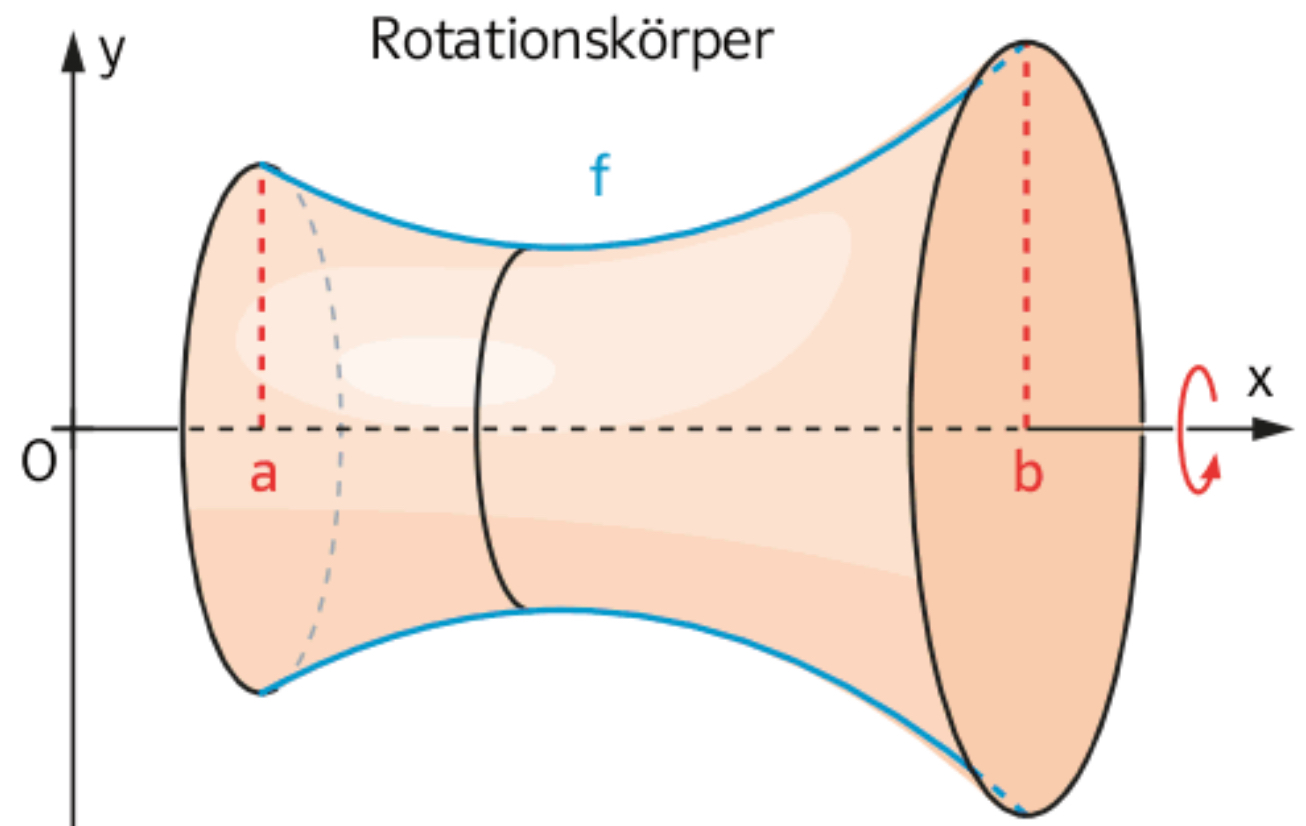
\includegraphics[width=4cm]{IMG_1121.jpg}
		\end{columns}
	\end{frame}
	
	\begin{frame}
		\section{Berechnung des Volumens}
		\frametitle{Berechnung des Volumens}
		\begin{block}{1. Schritt}
			\begin{itemize}
				\item Der Körper wird mit gleichbleibend Zylindern angenähert. Jeder Zylinder hat die Höhe $\Delta x$: $V_n = \pi \times (f(x_1))^2 \times \Delta x + \pi \times (f(x_2))^2 \times \Delta x +\ ...\ + \pi \times (f(x_n))^2 \times \Delta x$
				\item Diese Formel entspricht einer Summe wie $A_n$ beim Flächeninhalt, wenn man $g(x) = \pi \times (f(x))^2$ setzt. 
			\end{itemize}			
		\end{block}

		
		\begin{block}{2. Schritt}
			Grenzwert ($\lim_{n\to\infty} V_n$) entspricht dem Integral $\int_{a}^{b} g(x) dx = \int_{a}^{b} (\pi \times (f(x))^2) dx = \pi \int_{a}^{b} (f(x))^2 dx$
		\end{block}
	\end{frame}
	
	\begin{frame}
		\section{Übungsaufgabe}
		\frametitle{Übungsaufgabe}
		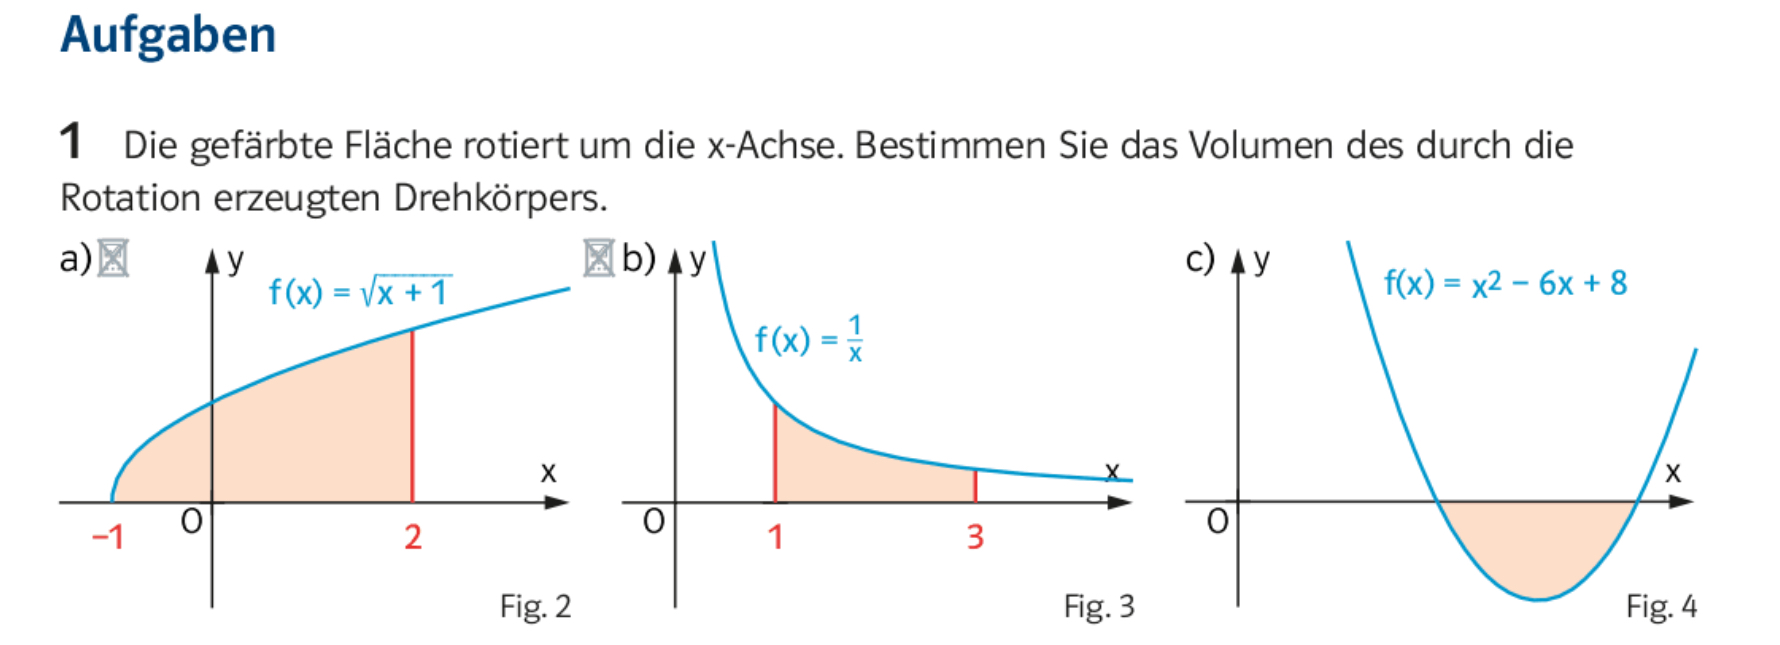
\includegraphics[width=11cm]{IMG_58408E42A4CB-1.JPEG}
	\end{frame}
	
	\section{Lösungen}
	\begin{frame}
		\frametitle{Lösung a)}
		\begin{block}{Rechnung}
			$V_n = \pi \times \int_{-1}^{2} (f(x))^2 dx$ \\
			$= \pi \times \int_{-1}^{2} (\sqrt{x+1})^2 dx = \Bigl[\frac{1}{2}x^2 + x\Bigl]_{-1}^{2}$ \\
			$= \pi \times \Bigl(4 - (-\frac{1}{2})\Bigl)$ \\
			$= \pi \times \frac{9}{2}$ \\
		\end{block}
	\end{frame}
	
	\begin{frame}
		\frametitle{Lösung b)}

		\begin{block}{Rechnung}	
			$V_n = \pi \times \int_{1}^{3}(f(x))^2 dx = \Bigl[F(3) - F(1)\Bigl]_{1}^{3}$ \\
			$= \pi \times \int_{1}^{3}(\frac{1}{x})^2 dx = \Bigl[F(3) - F(1)\Bigl]_{1}^{3}$ \\
			$= \pi \times \int_{1}^{3}(\frac{1}{x^2}) dx = \Bigl[F(3) - F(1)\Bigl]_{1}^{3}$ \\
			$= \pi \times (\frac{-1}{3}-(-1))$ \\
			$= \frac{2 \times \pi}{3}$ $\approx 2.0944$
		\end{block}

	\end{frame}
	
	\begin{frame}
		\frametitle{Lösung c)}
		\begin{block}{Rechnung}
			$f(x) = x^2 - 6x + 8$ \\
			\textbf{Nullstellen}: $f(x) = 0 \to x_1 = 2 \land x_2 = 4$ \\
			$\pi \times \int_{2}^{4}(f(x)^2) dx$ \\
			$= \frac{16\times\pi}{15}$
		\end{block}
	\end{frame}
	
	\section{Ende}
	\begin{frame}
		\centering
		\Huge{
			\textbf{Vielen Dank für Eure Aufmerksamkeit!}
		}
	\end{frame}

\end{document}